No existe una definición universalmente aceptada de lo que configura discurso de odio. En esta sección haremos un repaso muy breve de algunos tratados internacionales sobre la materia para intentar aproximarnos a este concepto, a la vez que también haremos un racconto de las definiciones utilizadas en trabajos dedicados a la construcción de datasets.

Un derecho que suele estar protegido por constituciones nacionales y tratados internacionales es el del derecho a la expresión. Por ejemplo, el Pacto de San José de Costa Rica (a la cual Argentina adhiere)\cite{humanos2018convencion} dice en su Artículo 13:

\begin{displayquote}[CADH, Artículo 13][]

    1. Toda persona tiene derecho a la libertad de pensamiento y de expresión.  Este derecho comprende la libertad de buscar, recibir y difundir informaciones e ideas de toda índole, sin consideración de fronteras, ya sea oralmente, por escrito o en forma impresa o artística, o por cualquier otro procedimiento de su elección.

    2. El ejercicio del derecho previsto en el inciso precedente no puede estar sujeto a previa censura sino a responsabilidades ulteriores, las que deben estar expresamente fijadas por la ley y ser necesarias para asegurar:

    a)  el respeto a los derechos o a la reputación de los demás, o

    b) la protección de la seguridad nacional, el orden público o la salud o la moral públicas.
\end{displayquote}

En Estados Unidos, la primer enmienda protege este derecho humano, mientras que en la Unión Europea, legislación similar ofrece protección a la libertad de expresión. Finalmente, la declaración universal de los derechos humanos de la ONU \todo{citation needed} menciona tanto en su preámbulo como en el artículo 19

\begin{displayquote}[Declaración Universal de los Derechos Humanos][ONU]
    Todo individuo tiene derecho a la libertad de opinión y de expresión; este derecho incluye el de no ser molestado a causa de sus opiniones, el de investigar y recibir informaciones y opiniones, y el de difundirlas, sin limitación de fronteras, por cualquier medio de expresión.
\end{displayquote}

Otro documento conocido como el Pacto Internacional de Derechos Civiles y Políticos (ICCPR por sus siglas en inglés) menciona

\begin{displayquote}[Artículo 19 de la ICCPR]
1. Nadie podrá ser molestado a causa de sus opiniones.

2. Toda persona tiene derecho a la libertad de expresión; este derecho comprende la libertad de buscar, recibir y difundir informaciones e ideas de toda índole, sin consideración de fronteras, ya sea oralmente, por escrito o en forma impresa o artística, o por cualquier otro procedimiento de su elección.

3. El ejercicio del derecho previsto en el párrafo 2 de este artículo entraña deberes y responsabilidades especiales. Por consiguiente, puede estar sujeto a ciertas restricciones, que deberán, sin embargo, estar expresamente fijadas por la ley y ser necesarias para:

a) Asegurar el respeto a los derechos o a la reputación de los demás;

b) La protección de la seguridad nacional, el orden público o la salud o la moral públicas.
\end{displayquote}

Sin embargo, y como mencionan estos dos últimos apartados, la libertad de expresión tiene un límite: el ejercicio de los derechos e igualdad ante la ley. Por ejemplo, el Artículo 1 del Pacto de San José de Costa Rica dice lo siguiente:

\begin{displayquote}[Pacto San José de Costa Rica, CADH][Artículo 1]
    1. Los Estados Partes en esta Convención se comprometen a respetar los derechos y libertades reconocidos en ella y a garantizar su libre y pleno ejercicio a toda persona que esté sujeta a su jurisdicción, sin discriminación alguna por motivos de raza, color, sexo, idioma, religión, opiniones políticas o de cualquier otra índole, origen nacional o social, posición económica, nacimiento o cualquier otra condición social.
\end{displayquote}

A su vez, la Declaración Universal de los Derechos Humanos en su Artículo 1:

\begin{displayquote}
    Todos los seres humanos nacen libres e iguales en dignidad y derechos y, dotados como están de razón y conciencia, deben comportarse fraternalmente los unos con los otros.
\end{displayquote}

Entonces, los Estados y otros organismos deben tomar medidas para poder asegurar el libre ejercicio de los derechos y la igualdad de todos sus miembros, aún cuando esto pueda significar una restricción en la libertad de expresión \cite{article192015}.


¿Qué es el discurso de odio entonces? Como hemos mencionado, no hay una definición universalmente aceptada. Repasemos algunas clasificaciones hechas en estos tratados para acercarnos un poco más a las características comunes que comparten.

Como vimos, el Pacto de San José de Costa Rica en su Artículo 1 habla del ejercicio de derechos sin discriminación alguna por varias razones, entre las que menciona raza, sexo, idioma, religión, política, nacionalidad, posición económica, entre otras. La Observación General 35 del Comité por la Eliminación de la Discriminación Racial de la ONU (CERD) considera que será discurso de odio, y debe ser tipificado penalmente:


\begin{displayquote}[Recomendación 35 del Comité por la Eliminación de la Discriminación Racial, CERD]

    a) Toda difusión de ideas basada en la superioridad o en el odio racial o étnico, por cualquier medio;

    b) La incitación al odio, el desprecio o la discriminación contra los miembros de un grupo por motivos de su raza, color, linaje, u origen nacional o étnico;

    c) Las amenazas o la incitación a la violencia contra personas o grupos por los motivos señalados en el apartado anterior;

    d) La expresión de insultos, burlas o calumnias contra personas o grupos, o la justificación del odio, el desprecio o la discriminación por los motivos señalados en el apartado b) anterior, cuando constituyan claramente incitación al odio o a la discriminación;

    e) La participación en organizaciones y actividades que promuevan e inciten a la discriminación racial.
\end{displayquote}

\citet{gagliardone2015countering} presenta un análisis de diversos organismos y sus definiciones de discurso de odio. En líneas generales, como se menciona en \citet{CIDH2015}, el concepto usualmente es referido a expresiones que incitan a tomar algún tipo de medida hostil contra una víctima o un grupo de personas, siendo esta perteneciente a un determinado grupo social definido por laguna característica. Dicho esto, podría delimitarse el discurso discriminatorio del discurso de odio por la componente de la promoción e instigación de la violencia; sin embargo, para los fines de este trabajo utilizaremos los términos indistintamente. Como se menciona también en \citet{CIDH2015}, aún cuando el discurso no contenga arengas ni incitaciones a cometer actos violentos, puede entenderse ese discurso como generador de un ambiente hostil y de intolerancia que termine promoviendo estos ataques físicos.


\citet{article192015} condensa muchas de estas definiciones de una manera succinta, desglosando esto en ``odio'' y ``discurso'':

\begin{displayquote}[Article 19: Hate Speech Toolkit]

    – Odio: emoción intensa e irracional de oprobio, enemistad y aborrecimiento hacia una persona o grupo de personas, por tener determinadas características protegidas (reconocidas en el derecho internacional), reales o percibidas. El “odio” es más que un mero prejuicio y debe ser discriminatorio. El odio es una muestra de un estado emocional u opinión y, por lo tanto, se diferencia de cualquier acto o acción que se haya llevado a cabo.
    – Discurso: cualquier expresión que vierta opiniones o ideas, que comparte una
    opinión o una idea interna con un público externo. Puede adoptar muchas
    formas: escrita, no-verbal, visual o artística y puede ser difundida en los
    medios, incluyendo Internet, material impreso, radio o televisión.
\end{displayquote}

%%
%%
%% Link
%% https://docs.google.com/drawings/d/149dpb2nrvmFgWZJYcrToAxO4M5n7JNQInfWd62kw3jc/edit
%%
%%

\begin{figure}[t]
    \centering
    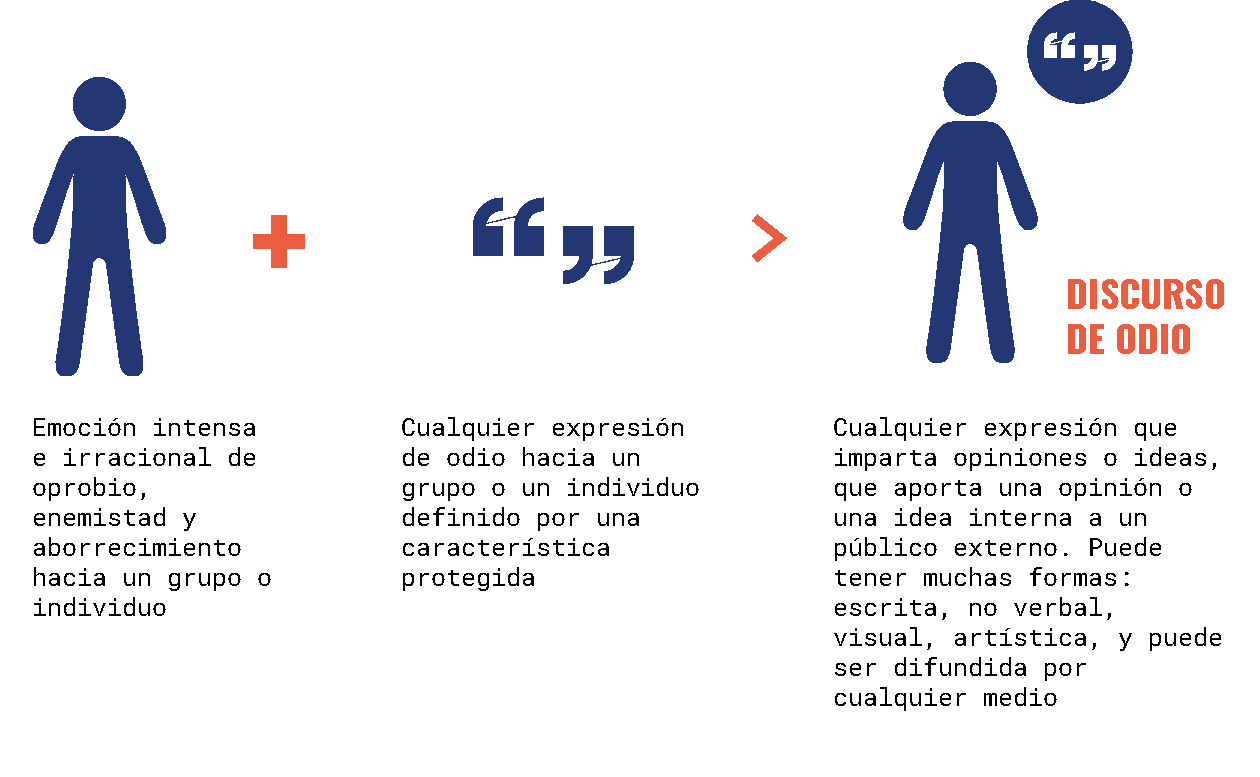
\includegraphics[width=\textwidth]{img/discurso_de_odio.pdf}
    \caption{Definición de discurso de odio de acuerdo al Toolkit de Article 19}
    \label{fig:hate_speech_definition_article_19}
\end{figure}


Entonces, puede entenderse como un discurso de cierta intensidad e irracionalidad que ataca a una persona o un grupo de personas por alguna característica históricamente vulnerada: por ser mujer, por su etnia, nacionalidad, religión, idioma, etc. La clave está en la combinación: un discurso irracional e intenso contra alguien que no posea una característica protegida no configura discurso de odio; por ejemplo, ataques a ciertas personas por ser periodistas. La figura \ref{fig:hate_speech_definition_article_19} ilustra esta definición.

No todo ataque a un individuo o una persona de algún colectivo discriminado es discurso de odio. En particular, en \citet{CIDH2015} se menciona en base al informe de la UNESCO sobre discurso de odio \citet{gagliardone2015countering} que:

\begin{displayquote}[]
    (...) el discurso de odio no puede abarcar ideas amplias y abstractas, tales como las visiones e ideologías políticas, la fe o las creencias personales. Tampoco se refiere simplemente a un insulto, expresión injuriosa o provocadora respecto de una persona. Así definido, el discurso de odio puede ser manipulado fácilmente para abarcar expresiones que puedan ser consideradas ofensivas por otras personas, particularmente por quienes están en el poder, lo que conduce a la indebida aplicación de la ley para restringir las expresiones críticas y disidentes. Asimismo, el discurso de odio tiene que distinguirse de aquellos “crímenes de odio” que se basan en conductas expresivas, como las amenazas y la violencia sexual, y que se encuentran fuera de cualquier protección del derecho a la libertad de expresión
\end{displayquote}

Como vemos, no sólamente es difusa la frontera fijada la característica sobre qué es discurso de odio o insultos, sino que incluso también es difícil definir qué característica es protegida o no. En el siguiente capítulo hablaremos más de esto al relatar cuáles fueron usadas a la hora de anotar nuestro dataset.

Si bien, como mencionamos, en cierta legislación se diferencia entre discurso discriminatorio y discurso de odio, para los fines de este trabajo utilizaremos ambas acepciones indistintamente. Cuando haya un llamado o una incitación a la violencia o algún tipo de represalia se hará explícita esta cuestión.
